\chapter{Arhitektura i dizajn sustava}
		
		\text{ Arhitektura se može podijeliti na četiri podsustava:}
		\begin{itemize}
			\item 	\text{Web poslužitelj}
			\item 	\text{Web aplikacija}
			\item 	\text{Baza podataka}
			\item 	\text{Domaćin za pohranu slika}
		\end{itemize}

			\begin{figure}[H]
				\includegraphics[scale=0.5]{slike/opis_arhitekture.png} %veličina slike u odnosu na originalnu datoteku i pozicija slike
				\centering
				\caption{Arhitektura sustava}
			\end{figure}
		\textbf{Web preglednik} je alat koji korisniku omogućava pregled web stranica i  svih sadržaja povezanih s isitima. Svaki web preglednik može prevesti kod web aplikacije. Korisnik putem web preglednika šalje zahtjeve na poslužitelj.

		\textbf{Web poslužitelj} ima zadaću vršiti komunikaciju između klijenta i aplikacije. Komunikacija se odvija pomoću HTTP protokola(\textit{Hyper Text Transfer Protocol}). Poslužitelj je ili pokretač web aplikacije, ili server na kojem je web aplikacija postavljena.

		\textbf{Web aplikacija} služi za obradu zahtjeva. Ovisno o zahtjevu, web aplikacija pristupa bazi podataka ili domaćinu za pohranu slika te korisniku vraća generirani HTML dokument koji je vidljiv u web pregledniku.

		Programski jezik koji je korišten za izradu web aplikacije je Pyhton za \textit{backend} i Javascript za \textit{frontend}. Preciznije za \textit{backend} dio koristi se Django, a za \textit{frontend} dio koristi se React. Time smo odvojili \textit{backend} za logiku i obradu podataka, a \textit{frontend} za komunikaciju s korisnikom. Django služi za upravljanje podacima te omogućava definiranje modela podataka i logike aplikacije. React služi za kreiranje korisničkog sučelja. Omogućava brzo i efikasno kreiranje dinamičkih i interaktivnih korisničkih sučelja. Razvojno okruženje u kojem radimo je Microsoft Visual Studio Code.

		\textbf{Domaćin za pohranu slika} je vanjski servis na koji se spremaju slike iz korsničkih zahtjeva poslanih iz web preglednika. Za to koristimo \url{https://imgur.com/}.


				
		\section{Baza podataka}
			
			
		\text{Za našu aplikaciju koristit ćemo relacijsku bazu podataka koja će nam olakšati modeliranje samog zadatka. 
		Relacijska baza podataka je baza podataka koja je organizirana u skup tablica koje su međusobno povezane. 
		Svaka tablica predstavlja jednu entitetnu klasu, a svaki redak tablice predstavlja jedan objekt dok stupci predstavljaju atribute. 
		Svaki objekt ima svoj jedinstveni identifikator koji se zove primarni ključ, a može imati i strane ključeve koji su referenca na primarni ključ nekog drugog objekta.
		Baza podataka se koristi za brzu i jednostavnu pohranu podataka koje naknadno možemo lako dohvatiti ili promijeniti.
		Baza podataka naše aplikacije sadrži slijedeće entitete: 
		}\\

		\begin{packed_item}
			\item  Korisnik
			\item  Pripada
			\item  Grupa
			\item  SpecijalizacijaRačunovođe
			\item  Dokument
			\item  Račun
			\item  Ponuda
			\item  InterniDokument
			\item  NedefiniraniDokument
			\item  Arhiva
			\item  RačunArhiviran
			\item  PonudaArhivirana
			\item  InterniDokumentArhiviran
			\item  NedefiniraniDokumentArhiviran
			\item  Artikl
			\item  NaRačunu
			\item  UPonudi
			\item  NaArhiviranomRačunu
			\item  UArhiviranojPonudi
		\end{packed_item}
		
			\subsection{Opis tablica}
			

				\textbf{Korisnik}: ovaj entitet sadrži sve informacije o korisniku aplikacije. Sadrži atribute: KorisnikId, Ime, Prezime, E-mail, Zaporka, KorisnickoIme, JeAdmin, ZadnjiLogin, JeAktivan, DatumZaposlenja. KorisnikId je primarni ključ.
				Veze s entitetom Korisnik su: One-to-many veza s entitetom Dokument preko atributa KorisnikId,
				One-to-many veza s entitetom Dokument preko atributa KorisnikId (ZaPotvrditiOdDirektoraKorisnikId),
				One-to-many veza s entitetom Dokument preko atributa KorisnikId (ZaPotvrditiOdRevizoraKorisnikId),
				One-to-many veza s entitetom Dokument preko atributa KorisnikId (ZaPotvrditiOdRačunovođeKorisnikId),
				One-to-many veza s entitetom Arhiva preko atributa KorisnikId,
				One-to-many veza s entitetom Arhiva preko atributa KorisnikId (PotvrdioRevizorKorisnikId),
				One-to-many veza s entitetom Arhiva preko atributa KorisnikId (PotvrdioRačunovođaKorisnikId),
				One-to-many veza s entitetom Arhiva preko atributa KorisnikId (PotvrdioDirektorKorisnikId),
				One-to-many veza s entitetom Pripada preko atributa KorisnikId,
				One-to-many veza s entitetom SpecijalizacijaRačunovođe preko atributa KorisnikId.\\
				
				
				\begin{longtblr}[
					label=none,
					entry=none
					]{
						width = \textwidth,
						colspec={|X[8,l]|X[6, l]|X[20, l]|}, 
						rowhead = 1,
					} %definicija širine tablice, širine stupaca, poravnanje i broja redaka naslova tablice
					\hline \SetCell[c=3]{c}{\textbf{Korisnik}}	 \\ \hline[3pt]
					\SetCell{LightGreen}KorisnikId & INT	&  	jedinstveni identifikator korisnika  	\\ \hline
					Ime	& VARCHAR &   ime korisnika	\\ \hline 
					Prezime & VARCHAR &  prezime korisnika \\ \hline 
					E-mail & VARCHAR	&  	E-mail korisnika	\\ \hline 
					Zaporka	& VARCHAR &   hash zaporke	\\ \hline 
					KorisnickoIme	& VARCHAR &   korisničko ime korisnika	\\ \hline 
					JeAdmin	& BOOLEAN &   oznaka je li korisnik admin aplikacije	\\ \hline 
					ZadnjiLogin	& DATETIME &   datum i vrijeme zadnjeg login-a korisnika	\\ \hline 
					JeAktivan	& BOOLEAN &   oznaka je li korisnik i dalje zaposlen	\\ \hline 
					DatumZaposlenja	& DATETIME &  datum i vrijeme kada je korisnik počeo raditi 	\\ \hline 
				\end{longtblr}

				\textbf{Pripada}: ovaj entitet sadrži sve informacije o tome kojem korisniku pripadaju koje grupe. Sadrži atribute: KorisnikId, GrupaId. KorisnikId i GrupaId su strani ključevi te ujedno i primarni ključ.
				Veze s entitetom Pripada su: Many-to-one veza s entitetom Korisnik preko atributa KorisnikId,
				Many-to-one veza s entitetom Grupa preko atributa GrupaId.\\
				
				
				\begin{longtblr}[
					label=none,
					entry=none
					]{
						width = \textwidth,
						colspec={|X[6,l]|X[6, l]|X[20, l]|}, 
						rowhead = 1,
					} %definicija širine tablice, širine stupaca, poravnanje i broja redaka naslova tablice
					\hline \SetCell[c=3]{c}{\textbf{Pripada}}	 \\ \hline[3pt]
					\SetCell{LightBlue}KorisnikId & INT	&  	jedinstveni identifikator korisnika (Korisnik.KorisnikId)  	\\ \hline
					\SetCell{LightBlue}GrupaId	& INT &   jedinstveni identifikator grupe (Grupa.GrupaId)	\\ \hline
				\end{longtblr}

				\textbf{Grupa}: ovaj entitet sadrži sve informacije o grupama. Sadrži atribute: GrupaId, ImeGrupe. GrupaId je primarni ključ.
				Veza s entitetom Grupa je: One-to-many veza s entitetom Pripada preko atributa GrupaId.\\
				
				
				\begin{longtblr}[
					label=none,
					entry=none
					]{
						width = \textwidth,
						colspec={|X[6,l]|X[6, l]|X[20, l]|}, 
						rowhead = 1,
					} %definicija širine tablice, širine stupaca, poravnanje i broja redaka naslova tablice
					\hline \SetCell[c=3]{c}{\textbf{Grupa}}	 \\ \hline[3pt]
					\SetCell{LightGreen}GrupaId & INT	&  	jedinstveni identifikator grupe  	\\ \hline
					imeGrupe	& VARCHAR &   naziv grupe	\\ \hline 
				\end{longtblr}

				\textbf{SpecijalizacijaRačunovođe}: ovaj entitet sadrži sve informacije o specijalizacijama računovođa. Sadrži atribute: SpecijalizacijaId, SpecijalizacijaIme, KorisnikId. SpecijalizacijaId je primarni ključ. KorisnikId je strani ključ.
				Veza s entitetom SpecijalizacijaRačunovođe su: Many-to-one veza s entitetom Korisnik preko atributa KorisnikId.\\
				
				
				\begin{longtblr}[
					label=none,
					entry=none
					]{
						width = \textwidth,
						colspec={|X[8,l]|X[6, l]|X[20, l]|}, 
						rowhead = 1,
					} %definicija širine tablice, širine stupaca, poravnanje i broja redaka naslova tablice
					\hline \SetCell[c=3]{c}{\textbf{SpecijalizacijaRačunovođe}}	 \\ \hline[3pt]
					\SetCell{LightGreen}SpecijalizacijaId & INT	&  	jedinstveni identifikator specijalizacije  	\\ \hline
					SpecijalizacijaIme	& VARCHAR &  naziv specijalizacije 	\\ \hline 
					\SetCell{LightBlue}KorisnikId	& INT &   jedinstveni identifikator računovođe koji je specijaliziran za određenu vrstu dokumenata (Korisnik.KorisnikId)	\\ \hline
				\end{longtblr}

				\textbf{Dokument}: ovaj entitet sadrži sve informacije o dokumentima. Sadrži atribute: DokumentId, TekstDokumenta, LinkSlike, VrijemeSkeniranja, PotpisaoDirektor, PotvrdioRevizor, PregledaoRačunovođa, KorisnikId, ZaPotvrditiOdDirektoraKorisnikId, ZaPotvrditiOdRevizoraKorisnikId, ZaPotvrditiOdRačunovođeKorisnikId. DokumentId je primarni ključ. KorisnikId, ZaPotvrditiOdDirektoraKorisnikId, ZaPotvrditiOdRevizoraKorisnikId, ZaPotvrditiOdRačunovođeKorisnikId su strani ključevi.
				Veze s entitetom Dokument su: Many-to-one veza s entitetom Korisnik preko atributa KorisnikId,
				Many-to-one veza s entitetom Korisnik preko atributa KorisnikId (ZaPotvrditiOdDirektoraKorisnikId),
				Many-to-one veza s entitetom Korisnik preko atributa KorisnikId (ZaPotvrditiOdRevizoraKorisnikId),
				Many-to-one veza s entitetom Korisnik preko atributa KorisnikId (ZaPotvrditiOdRačunovođeKorisnikId),
				One-to-one veza s entitetom Račun preko atributa DokumentId,
				One-to-one veza s entitetom Ponuda preko atributa DokumentId,
				One-to-one veza s entitetom InterniDokument preko atributa DokumentId,
				One-to-one veza s entitetom NedefiniraniDokument preko atributa DokumentId.
				
				
				\begin{longtblr}[
					label=none,
					entry=none
					]{
						width = \textwidth,
						colspec={|X[30,l]|X[8, l]|X[20, l]|}, 
						rowhead = 1,
					} %definicija širine tablice, širine stupaca, poravnanje i broja redaka naslova tablice
					\hline \SetCell[c=3]{c}{\textbf{Dokument}}	 \\ \hline[3pt]
					\SetCell{LightGreen}DokumentId & INT	&  	jedinstveni identifikator dokumenta  	\\ \hline
					TekstDokumenta	& VARCHAR &   tekst skeniranog dokumenta	\\ \hline 
					LinkSlike & VARCHAR &  poveznica s posluzitelja na kojem se nalazi spremljena slika dokumenta\\ \hline 
					VrijemeSkeniranja & DATETIME	&  	datum i vrijeme kada je napravljeno skeniranje slike dokumenta	\\ \hline 
					PotpisaoDirektor & BOOLEAN &  oznaka je li direktor potpisao dokument \\ \hline
					PotvrdioRevizor & BOOLEAN &  oznaka je li revizor potvrdio dokument \\ \hline
					PregledaoRačunovođa & BOOLEAN &  oznaka je li računovođa pregledao dokument \\ \hline
					\SetCell{LightBlue} KorisnikId	& INT &   jedinstveni identifikator korisnika koji je skenirao dokument(Korisnik.KorisnikId)	\\ \hline 
					\SetCell{LightBlue} ZaPotvrditiOdDirektoraKorisnikId	& INT &   jedinstveni identifikator direktora koji mora potvrditi dokument (Korisnik.KorisnikId)	\\ \hline
					\SetCell{LightBlue} ZaPotvrditiOdRevizoraKorisnikId	& INT &   jedinstveni identifikator revizora koji mora potvrditi dokument (Korisnik.KorisnikId)	\\ \hline
					\SetCell{LightBlue} ZaPotvrditiOdRačunovođeKorisnikId	& INT &   jedinstveni identifikator računovođe koji mora potvrditi dokument (Korisnik.KorisnikId)	\\ \hline
				\end{longtblr}

				\textbf{Račun}: ovaj entitet sadrži sve informacije o računima. Sadrži atribute: DokumentId, UkupnaCijena, ImeKlijenta. DokumentId je strani ključ.
				Veze s entitetom Račun su: One-to-one veza s entitetom Dokument preko atributa DokumentId,
				One-to-many veza s entitetom NaRačunu preko atributa DokumentId.
				
				
				\begin{longtblr}[
					label=none,
					entry=none
					]{
						width = \textwidth,
						colspec={|X[6,l]|X[6, l]|X[20, l]|}, 
						rowhead = 1,
					} %definicija širine tablice, širine stupaca, poravnanje i broja redaka naslova tablice
					\hline \SetCell[c=3]{c}{\textbf{Račun}}	 \\ \hline[3pt]
					\SetCell{LightBlue}DokumentId & INT	&  	jedinstveni identifikator dokumenta (Dokument.DokumentId)  	\\ \hline
					UkupnaCijena	& DECIMAL &   ukupna cijena svih artikala na računu	\\ \hline 
					ImeKlijenta & VARCHAR &  ime klijenta \\ \hline 
				\end{longtblr}

				\textbf{Ponuda}: ovaj entitet sadrži sve informacije o ponudama. Sadrži atribute: DokumentId, UkupnaCijena. DokumentId je strani ključ.
				Veze s entitetom Ponuda su: One-to-one veza s entitetom Dokument preko atributa DokumentId,
				One-to-many veza s entitetom UPonudi preko atributa DokumentId.
				
				
				\begin{longtblr}[
					label=none,
					entry=none
					]{
						width = \textwidth,
						colspec={|X[6,l]|X[6, l]|X[20, l]|}, 
						rowhead = 1,
					} %definicija širine tablice, širine stupaca, poravnanje i broja redaka naslova tablice
					\hline \SetCell[c=3]{c}{\textbf{Ponuda}}	 \\ \hline[3pt]
					\SetCell{LightBlue}DokumentId & INT	&  	jedinstveni identifikator dokumenta (Dokument.DokumentId)  	\\ \hline
					UkupnaCijena	& DECIMAL &   ukupna cijena svih artikala u ponudi	\\ \hline
				\end{longtblr}

				\textbf{InterniDokument}: ovaj entitet sadrži sve informacije o internim dokumentima. Sadrži atribut: DokumentId. DokumentId je strani ključ.
				Veze s entitetom InterniDokument su: One-to-one veza s entitetom Dokument preko atributa DokumentId.
				
				
				\begin{longtblr}[
					label=none,
					entry=none
					]{
						width = \textwidth,
						colspec={|X[6,l]|X[6, l]|X[20, l]|}, 
						rowhead = 1,
					} %definicija širine tablice, širine stupaca, poravnanje i broja redaka naslova tablice
					\hline \SetCell[c=3]{c}{\textbf{InterniDokument}}	 \\ \hline[3pt]
					\SetCell{LightBlue}DokumentId & INT	&  	jedinstveni identifikator dokumenta (Dokument.DokumentId)  	\\ \hline
				\end{longtblr}

				\textbf{NedefiniraniDokument}: ovaj entitet sadrži sve informacije o nedefiniranim dokumentima. Sadrži atribut: DokumentId. DokumentId je strani ključ.
				Veze s entitetom NedefiniraniDokument su: One-to-one veza s entitetom Dokument preko atributa DokumentId.
				
				
				\begin{longtblr}[
					label=none,
					entry=none
					]{
						width = \textwidth,
						colspec={|X[6,l]|X[6, l]|X[20, l]|}, 
						rowhead = 1,
					} %definicija širine tablice, širine stupaca, poravnanje i broja redaka naslova tablice
					\hline \SetCell[c=3]{c}{\textbf{NedefiniraniDokument}}	 \\ \hline[3pt]
					\SetCell{LightBlue}DokumentId & INT	&  	jedinstveni identifikator dokumenta (Dokument.DokumentId)  	\\ \hline
				\end{longtblr}

				\textbf{Arhiva}: ovaj entitet sadrži sve informacije o arhiviranim dokumentima. Sadrži atribute: ArhivaId, TekstDokumenta, LinkSlike, VrijemeSkeniranja, DokumentId, VrijemeArhiviranja, PotpisaoDirektor, PotvrdioRevizor, PregledaoRačunovođa, KorisnikId, ZaPotvrditiOdDirektoraKorisnikId, ZaPotvrditiOdRevizoraKorisnikId, ZaPotvrditiOdRačunovođeKorisnikId. ArhivaId je primarni ključ. KorisnikId, ZaPotvrditiOdDirektoraKorisnikId, ZaPotvrditiOdRevizoraKorisnikId, ZaPotvrditiOdRačunovođeKorisnikId su strani ključevi.
				Veze s entitetom Arhiva su: Many-to-one veza s entitetom Korisnik preko atributa KorisnikId,
				Many-to-one veza s entitetom Korisnik preko atributa KorisnikId (ZaPotvrditiOdDirektoraKorisnikId),
				Many-to-one veza s entitetom Korisnik preko atributa KorisnikId (ZaPotvrditiOdRevizoraKorisnikId),
				Many-to-one veza s entitetom Korisnik preko atributa KorisnikId (ZaPotvrditiOdRačunovođeKorisnikId),
				One-to-one veza s entitetom RačunArhiviran preko atributa ArhivaId,
				One-to-one veza s entitetom PonudaArhivirana preko atributa ArhivaId,
				One-to-one veza s entitetom InterniDokumentArhiviran preko atributa ArhivaId,
				One-to-one veza s entitetom NedefiniraniDokumentArhiviran preko atributa ArhivaId.

				
				
				\begin{longtblr}[
					label=none,
					entry=none
					]{
						width = \textwidth,
						colspec={|X[30,l]|X[10, l]|X[20, l]|}, 
						rowhead = 1,
					} %definicija širine tablice, širine stupaca, poravnanje i broja redaka naslova tablice
					\hline \SetCell[c=3]{c}{\textbf{Arhiva}}	 \\ \hline[3pt]
					\SetCell{LightGreen}ArhivaId & INT	&  	jedinstveni identifikator arhive  	\\ \hline
					TekstDokumenta	& VARCHAR &   tekst arhiviranog dokumenta	\\ \hline 
					LinkSlike & VARCHAR &  poveznica s posluzitelja na kojem se nalazi spremljena slika arhiviranog dokumenta \\ \hline 
					VrijemeSkeniranja & DATETIME	&  	datum i vrijeme kada je napravljeno skeniranje slike arhiviranog dokumenta	\\ \hline 
					DokumentId & INT &  jedinstveni identifikator dokumenta  \\ \hline
					VrijemeArhiviranja & DATETIME &  datum i vrijeme kada je dokument arhiviran \\ \hline
					PotpisaoDirektor & BOOLEAN &  oznaka je li direktor potpisao arhivirani dokument \\ \hline
					PotvrdioRevizor & BOOLEAN &  oznaka je li revizor potvrdio arhivirani dokument \\ \hline
					PregledaoRačunovođa & BOOLEAN &  oznaka je li računovođa pregledao arhivirani dokument \\ \hline
					\SetCell{LightBlue} KorisnikId	& INT &   jedinstveni identifikator korisnika koji je skenirao arhivirani dokument(Korisnik.KorisnikId)	\\ \hline 
					\SetCell{LightBlue} ZaPotvrditiOdDirektoraKorisnikId	& INT &   jedinstveni identifikator direktora koji je morao potvrditi dokument prije arhiviranja(Korisnik.KorisnikId)	\\ \hline
					\SetCell{LightBlue} ZaPotvrditiOdRevizoraKorisnikId	& INT &   jedinstveni identifikator revizora koji je morao potvrditi dokument prije arhiviranja (Korisnik.KorisnikId)	\\ \hline
					\SetCell{LightBlue} ZaPotvrditiOdRačunovođeKorisnikId	& INT &   jedinstveni identifikator računovođe koji je morao potvrditi dokument prije arhiviranja (Korisnik.KorisnikId)	\\ \hline
				\end{longtblr}

				\textbf{RačunArhiviran}: ovaj entitet sadrži sve informacije o računima koji su arhivirani. Sadrži atribute: ArhivaId, UkupnaCijena, ImeKlijenta. ArhivaId je strani ključ.
				Veze s entitetom Račun su: One-to-one veza s entitetom Arhiva preko atributa ArhivaId,
				One-to-many veza s entitetom NaArhiviranomRačunu preko atributa ArhivaId.
				
				
				\begin{longtblr}[
					label=none,
					entry=none
					]{
						width = \textwidth,
						colspec={|X[6,l]|X[6, l]|X[20, l]|}, 
						rowhead = 1,
					} %definicija širine tablice, širine stupaca, poravnanje i broja redaka naslova tablice
					\hline \SetCell[c=3]{c}{\textbf{RačunArhiviran}}	 \\ \hline[3pt]
					\SetCell{LightBlue}ArhivaId & INT	&  	jedinstveni identifikator arhive (Arhiva.ArhivaId)  	\\ \hline
					UkupnaCijena	& DECIMAL &   ukupna cijena svih artikala na arhiviranom računu	\\ \hline 
					ImeKlijenta & VARCHAR &  ime klijenta na arhiviranom računu\\ \hline 
				\end{longtblr}

				\textbf{PonudaArhivirana}: ovaj entitet sadrži sve informacije o ponudama koje su arhivirane. Sadrži atribute: ArhivaId, UkupnaCijena. ArhivaId je strani ključ.
				Veze s entitetom Ponuda su: One-to-one veza s entitetom Arhiva preko atributa ArhivaId,
				One-to-many veza s entitetom UArhiviranojPonudi preko atributa ArhivaId.
				
				
				\begin{longtblr}[
					label=none,
					entry=none
					]{
						width = \textwidth,
						colspec={|X[6,l]|X[6, l]|X[20, l]|}, 
						rowhead = 1,
					} %definicija širine tablice, širine stupaca, poravnanje i broja redaka naslova tablice
					\hline \SetCell[c=3]{c}{\textbf{PonudaArhivirana}}	 \\ \hline[3pt]
					\SetCell{LightBlue}ArhivaId & INT	&  	jedinstveni identifikator arhive (Arhiva.ArhivaId)   	\\ \hline
					UkupnaCijena	& DECIMAL &   ukupna cijena svih artikala u arhiviranoj ponudi	\\ \hline
				\end{longtblr}

				\textbf{InterniDokumentArhiviran}: ovaj entitet sadrži sve informacije o internim dokumentima koji su arhivirani. Sadrži atribut: ArhivaId. ArhivaId je strani ključ.
				Veze s entitetom InterniDokument su: One-to-one veza s entitetom Arhiva preko atributa ArhivaId.
				
				
				\begin{longtblr}[
					label=none,
					entry=none
					]{
						width = \textwidth,
						colspec={|X[6,l]|X[6, l]|X[20, l]|}, 
						rowhead = 1,
					} %definicija širine tablice, širine stupaca, poravnanje i broja redaka naslova tablice
					\hline \SetCell[c=3]{c}{\textbf{InterniDokumentArhiviran}}	 \\ \hline[3pt]
					\SetCell{LightBlue}ArhivaId & INT	&  	jedinstveni identifikator arhive (Arhiva.ArhivaId)  	\\ \hline
				\end{longtblr}

				\textbf{NedefiniraniDokumentArhiviran}: ovaj entitet sadrži sve informacije o nedefiniranim dokumentima koji su arhivirani. Sadrži atribut: ArhivaId. ArhivaId je strani ključ.
				Veze s entitetom NedefiniraniDokument su: One-to-one veza s entitetom Arhiva preko atributa ArhivaId.
				
				
				\begin{longtblr}[
					label=none,
					entry=none
					]{
						width = \textwidth,
						colspec={|X[6,l]|X[6, l]|X[20, l]|}, 
						rowhead = 1,
					} %definicija širine tablice, širine stupaca, poravnanje i broja redaka naslova tablice
					\hline \SetCell[c=3]{c}{\textbf{NedefiniraniDokumentArhiviran}}	 \\ \hline[3pt]
					\SetCell{LightBlue}ArhivaId & INT	&  	jedinstveni identifikator arhive (Arhiva.ArhivaId)  	\\ \hline
				\end{longtblr}

				\textbf{Artikl}: ovaj entitet sadrži sve informacije o artiklima. Sadrži atribute: ImeArtikla, Cijena. ImeArtikla je primarni ključ.
				Veze s entitetom Artikl su: One-to-many veza s entitetom NaRačunu preko atributa ImeArtikla,
				One-to-many veza s entitetom UPonudi preko atributa ImeArtikla,
				One-to-many veza s entitetom NaArhiviranomRačunu preko atributa ImeArtikla,
				One-to-many veza s entitetom UArhiviranojPonudi preko atributa ImeArtikla.
				
				
				\begin{longtblr}[
					label=none,
					entry=none
					]{
						width = \textwidth,
						colspec={|X[6,l]|X[6, l]|X[20, l]|}, 
						rowhead = 1,
					} %definicija širine tablice, širine stupaca, poravnanje i broja redaka naslova tablice
					\hline \SetCell[c=3]{c}{\textbf{Artikl}}	 \\ \hline[3pt]
					\SetCell{LightGreen}ImeArtikla & VARCHAR	&  	jedinstveno ime artikla  	\\ \hline
					Cijena	& DECIMAL &   cijena artikla	\\ \hline 
				\end{longtblr}

				\textbf{NaRačunu}: ovaj entitet sadrži sve informacije o tome koji artikli se nalaze na računu. Sadrži atribute: DokumentId, ImeArtikla. DokumentId i ImeArtikla su strani ključevi.
				Veze s entitetom NaRačunu su: Many-to-one veza s entitetom Račun preko atributa DokumentId,
				Many-to-one veza s entitetom Artikl preko atributa ImeArtikla.
				
				
				\begin{longtblr}[
					label=none,
					entry=none
					]{
						width = \textwidth,
						colspec={|X[6,l]|X[6, l]|X[20, l]|}, 
						rowhead = 1,
					} %definicija širine tablice, širine stupaca, poravnanje i broja redaka naslova tablice
					\hline \SetCell[c=3]{c}{\textbf{NaRačunu}}	 \\ \hline[3pt]
					\SetCell{LightBlue}DokumentId & INT	&  	jedinstveni identifikator dokumenta (Dokument.DokumentId)  	\\ \hline
					\SetCell{LightBlue}ImeArtikla & VARCHAR	&  	jedinstveno ime artikla (Artikl.ImeArtikla)  	\\ \hline
				\end{longtblr}

				\textbf{UPonudi}: ovaj entitet sadrži sve informacije o tome koji artikli se nalaze u ponudi. Sadrži atribute: DokumentId, ImeArtikla. DokumentId i ImeArtikla su strani ključevi.
				Veze s entitetom UPonudi su: Many-to-one veza s entitetom Ponuda preko atributa DokumentId,
				Many-to-one veza s entitetom Artikl preko atributa ImeArtikla.
				
				
				\begin{longtblr}[
					label=none,
					entry=none
					]{
						width = \textwidth,
						colspec={|X[6,l]|X[6, l]|X[20, l]|}, 
						rowhead = 1,
					} %definicija širine tablice, širine stupaca, poravnanje i broja redaka naslova tablice
					\hline \SetCell[c=3]{c}{\textbf{UPonudi}}	 \\ \hline[3pt]
					\SetCell{LightBlue}DokumentId & INT	&  	jedinstveni identifikator dokumenta (Dokument.DokumentId)  	\\ \hline
					\SetCell{LightBlue}ImeArtikla & VARCHAR	&  	jedinstveno ime artikla (Artikl.ImeArtikla)  	\\ \hline
				\end{longtblr}

				\textbf{NaArhiviranomRačunu}: ovaj entitet sadrži sve informacije o tome koji artikli se nalaze na arhiviranom računu. Sadrži atribute: ArhivaId, ImeArtikla. ArhivaId i ImeArtikla su strani ključevi.
				Veze s entitetom NaArhiviranomRačunu su: Many-to-one veza s entitetom RačunArhiviran preko atributa ArhivaId,
				Many-to-one veza s entitetom Artikl preko atributa ImeArtikla.
				
				
				\begin{longtblr}[
					label=none,
					entry=none
					]{
						width = \textwidth,
						colspec={|X[6,l]|X[6, l]|X[20, l]|}, 
						rowhead = 1,
					} %definicija širine tablice, širine stupaca, poravnanje i broja redaka naslova tablice
					\hline \SetCell[c=3]{c}{\textbf{NaArhiviranomRačunu}}	 \\ \hline[3pt]
					\SetCell{LightBlue}ArhivaId & INT	&  	jedinstveni identifikator arhive (Arhiva.ArhivaId)  	\\ \hline
					\SetCell{LightBlue}ImeArtikla & VARCHAR	&  	jedinstveno ime artikla (Artikl.ImeArtikla)  	\\ \hline
				\end{longtblr}

				\textbf{UArhiviranojPonudi}: ovaj entitet sadrži sve informacije o tome koji artikli se nalaze u arhiviranoj ponudi. Sadrži atribute: ArhivaId, ImeArtikla. ArhivaId i ImeArtikla su strani ključevi.
				Veze s entitetom UArhiviranojPonudi su: Many-to-one veza s entitetom PonudaArhivirana preko atributa ArhivaId,
				Many-to-one veza s entitetom Artikl preko atributa ImeArtikla.
				
				
				\begin{longtblr}[
					label=none,
					entry=none
					]{
						width = \textwidth,
						colspec={|X[6,l]|X[6, l]|X[20, l]|}, 
						rowhead = 1,
					} %definicija širine tablice, širine stupaca, poravnanje i broja redaka naslova tablice
					\hline \SetCell[c=3]{c}{\textbf{UArhiviranojPonudi}}	 \\ \hline[3pt]
					\SetCell{LightBlue}ArhivaId & INT	&  	jedinstveni identifikator arhive (Arhiva.ArhivaId)  	\\ \hline
					\SetCell{LightBlue}ImeArtikla & VARCHAR	&  	jedinstveno ime artikla (Artikl.ImeArtikla)  	\\ \hline
				\end{longtblr}
				
				
			
			\subsection{Dijagram baze podataka}

			\begin{figure}[H]
				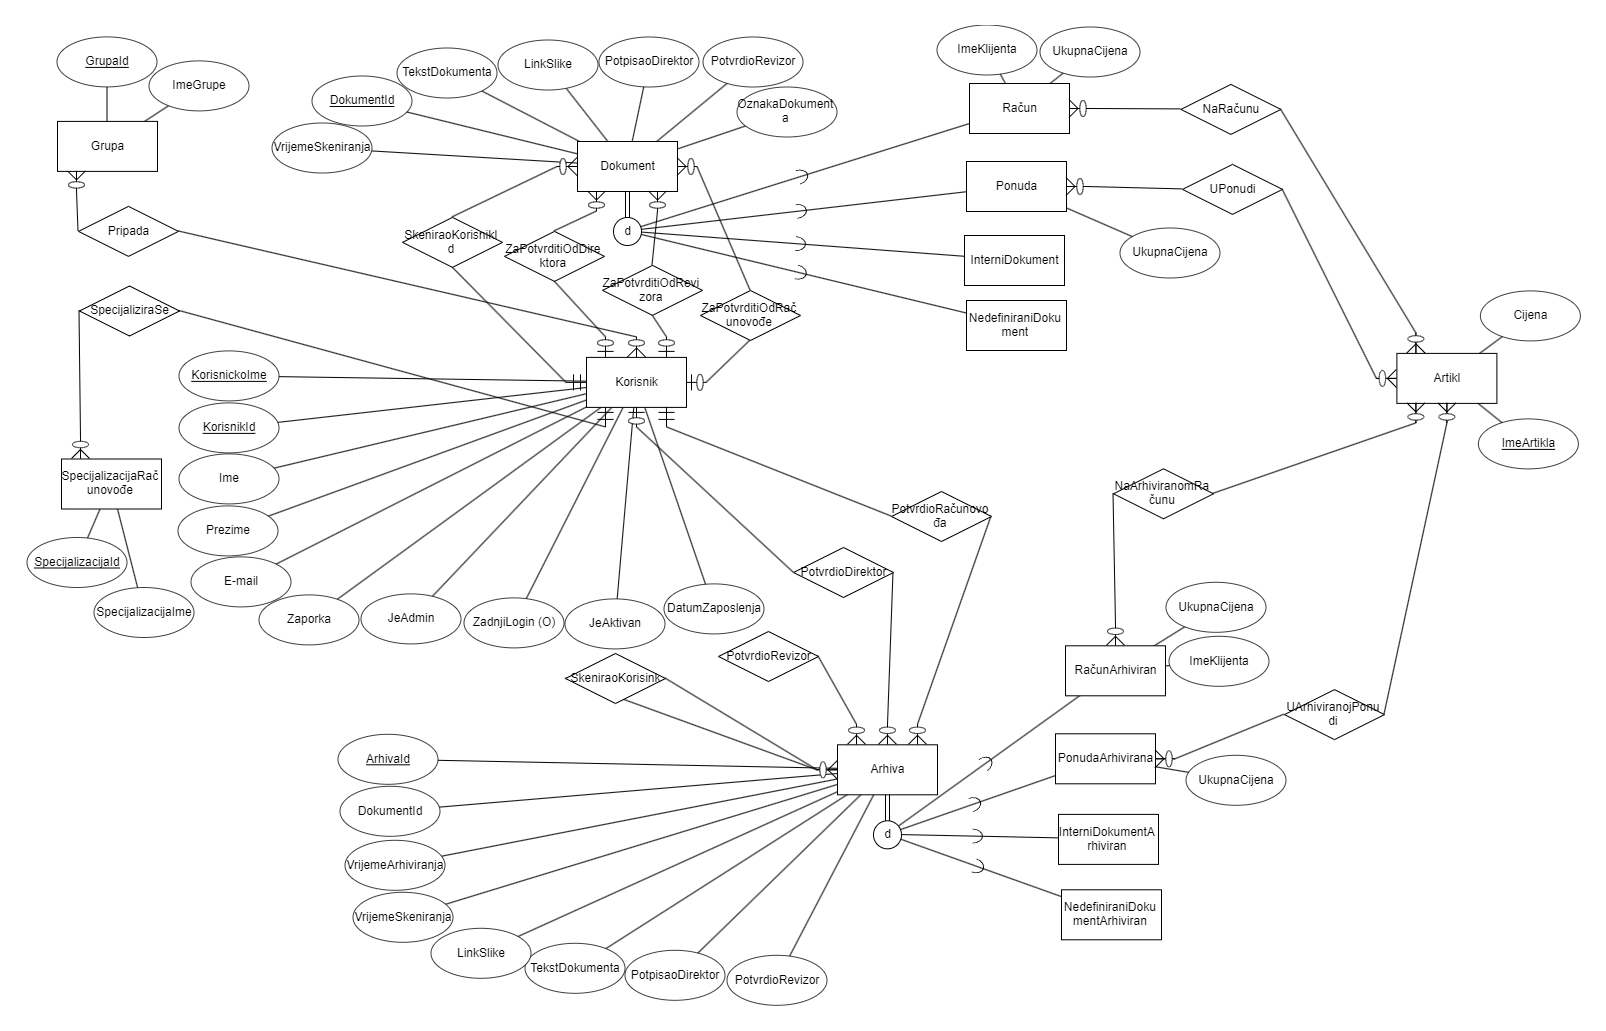
\includegraphics[width=\textwidth]{slike/ER_dijagram.png} %veličina u odnosu na širinu linije
				\caption{ER dijagram baze podataka}
				\label{fig:er_diagram} %label mora biti drugaciji za svaku sliku
			\end{figure}

			\begin{figure}[H]
				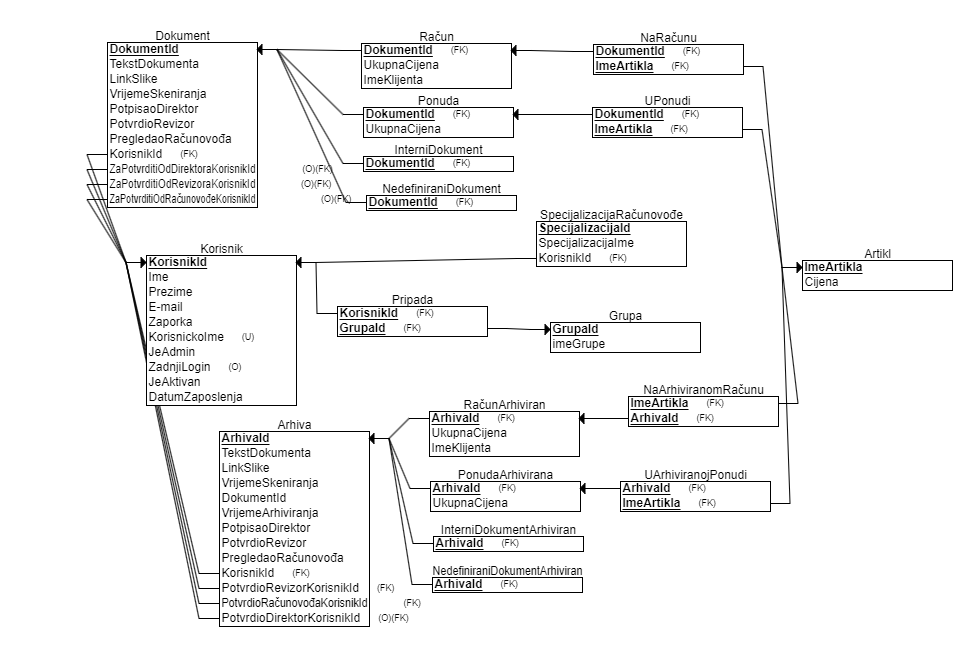
\includegraphics[width=\textwidth]{slike/Relacijska_shema.png} %veličina u odnosu na širinu linije
				\caption{Relacijska shema baze podataka}
				\label{fig:relacijska_shema} %label mora biti drugaciji za svaku sliku
			\end{figure}

			\eject
			
			
		\section{Dijagram razreda}
		
			Na dijagramu razreda Models (slika 4.4) prikazani su razredi unutar datoteke models.py te
			odnosi među njima. U datoteci postoji ukupno 12 razreda. Dokument je nadrazred 4 od tih razreda, a Arhiva
			je također nadrazred 4 od tih razreda.
			\newline
			Dijagram razreda Permissions (slika 4.5) prikazuje razred Permissions,
			koji je nadrazred razredima PripadaDirektorima, PripadaRačunovođama i PripadaRevizorima. Ti se
			razredi nalaze unutar datoteke permissions.py te definiraju kojoj grupi korisnik mora pripadati
			da bi mogao koristiti određeni prikaz web-aplikacije.
			\newline
			Razred Views nalazi se unutar datoteke views.py, u kojoj se također nalazi i razred
			MyTokenObtainPairSerializer kojemu je Views nadrazred. Views koristi taj razred kako bi
			serveru bilo preneseno koje dozvole su prisutne tijekom pokušaja pristupa aplikaciji.
			Na dijagramu razreda Views (slika 4.6) prikazan je odnos između ta dva razreda. 
			
			\begin{figure}[H]
				\
				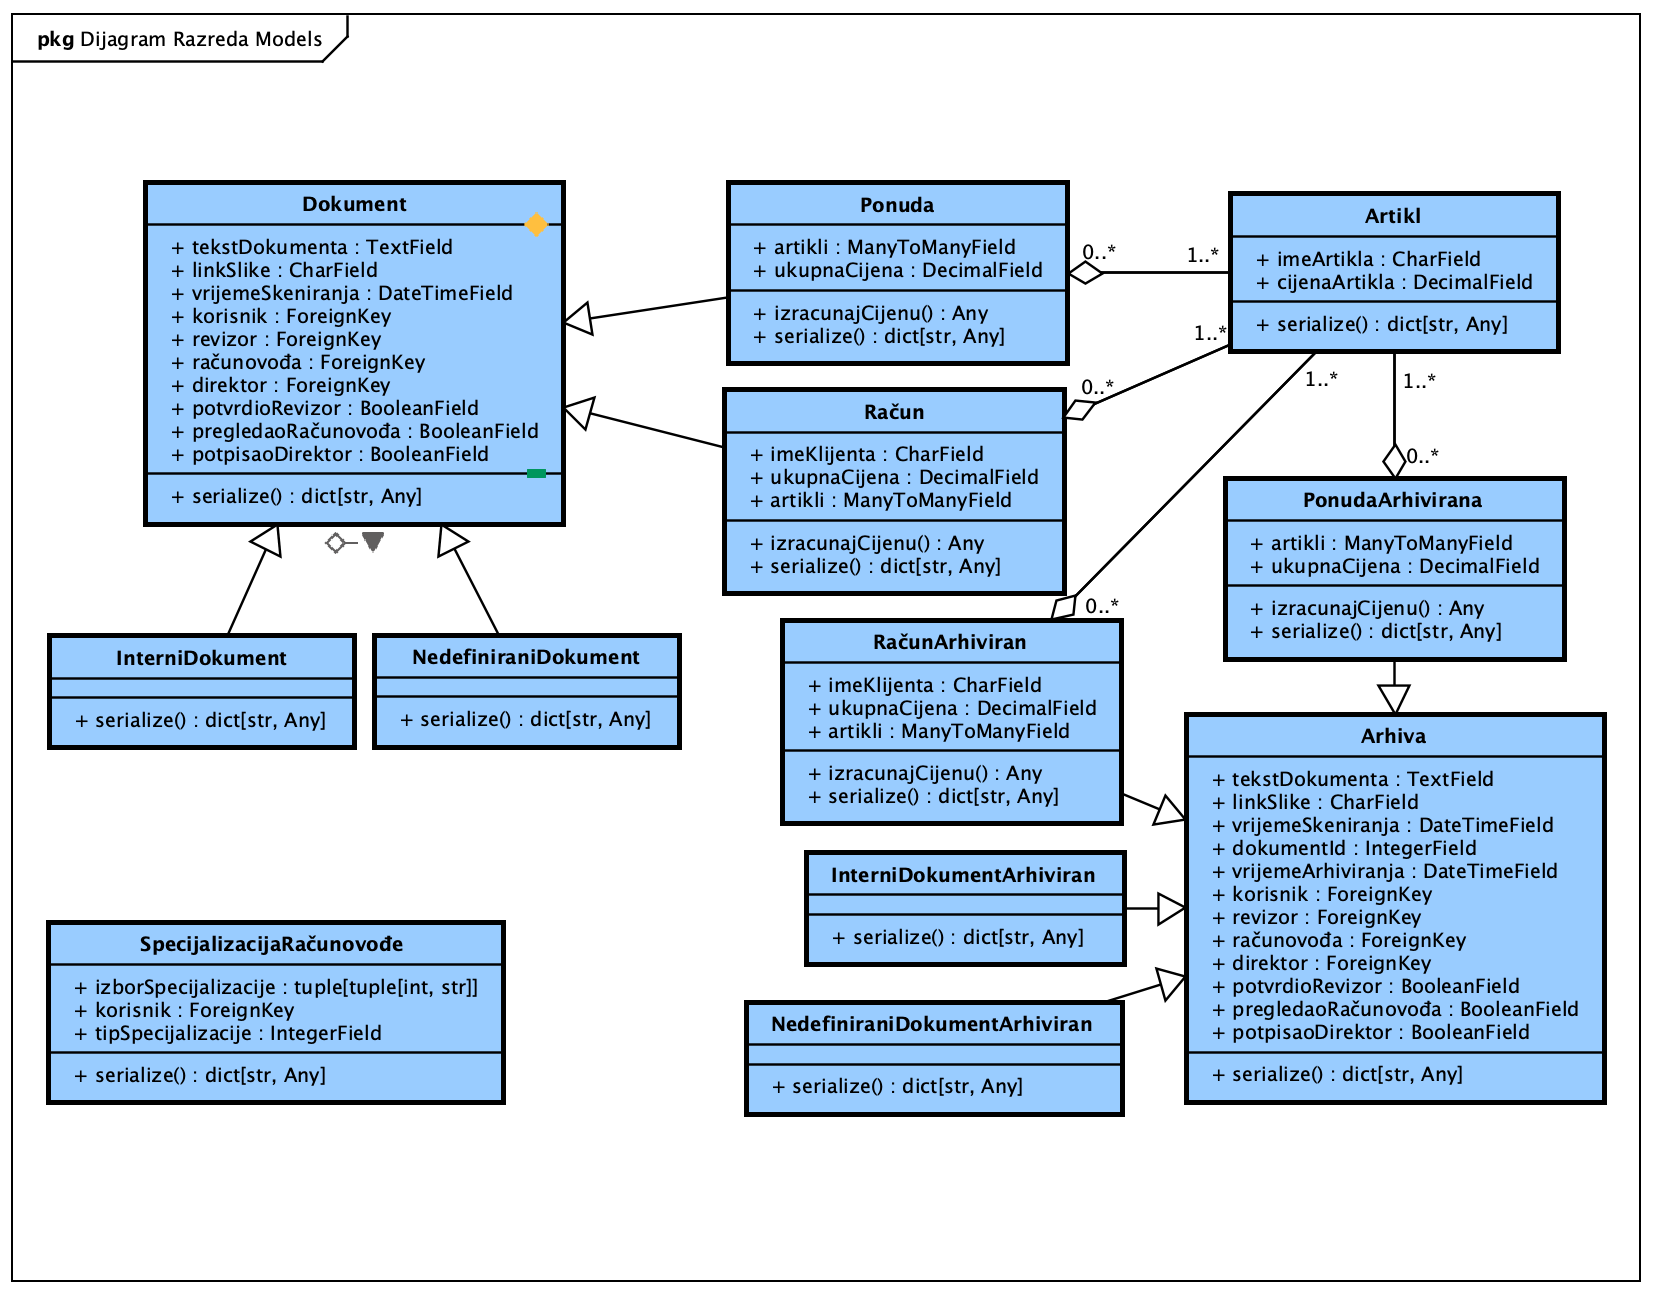
\includegraphics[width=\textwidth]{slike/Class_Models.png}
				\caption{Dijagram razreda - dio Models}
				\label{fig:class_models}
			\end{figure}

			\begin{figure}[H]
				\
				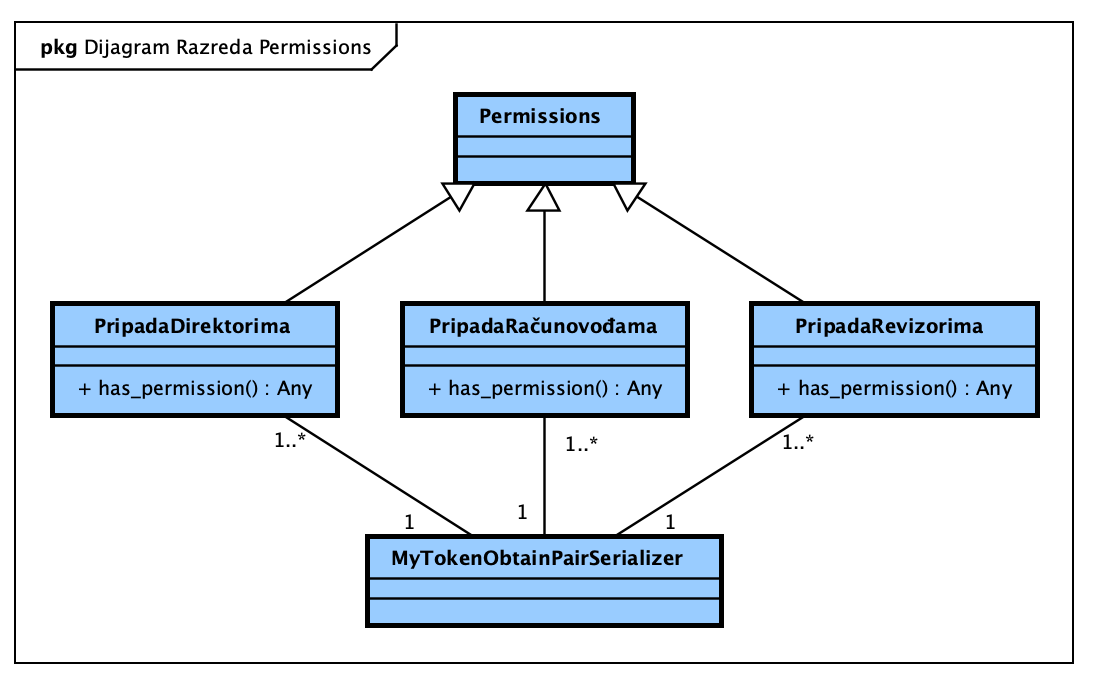
\includegraphics[width=\textwidth]{slike/Class_Permissions.png}
				\caption{Dijagram razreda - dio Permissions}
				\label{fig:class_permissions}
			\end{figure}

			\begin{figure}[H]
				\
				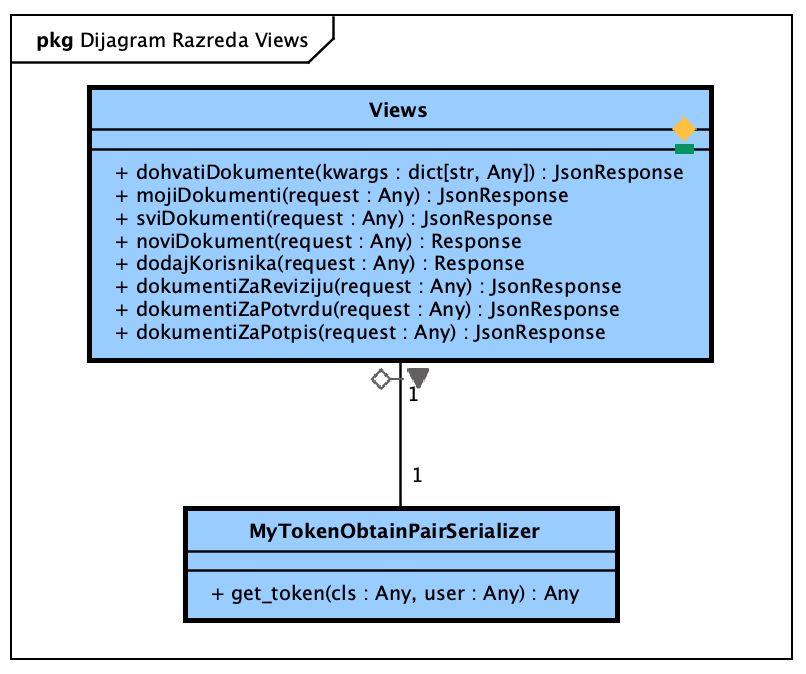
\includegraphics[width=\textwidth]{slike/Class_Views.png}
				\caption{Dijagram razreda - dio Views}
				\label{fig:class_views}
			\end{figure}

			\textbf{\textit{dio 2. revizije}}\\			
			
			\textit{Prilikom druge predaje projekta dijagram razreda i opisi moraju odgovarati stvarnom stanju implementacije}
			
			
			
			\eject
		
		\section{Dijagram stanja}
			
			
			\textbf{\textit{dio 2. revizije}}\\
			
			\textit{Potrebno je priložiti dijagram stanja i opisati ga. Dovoljan je jedan dijagram stanja koji prikazuje \textbf{značajan dio funkcionalnosti} sustava. Na primjer, stanja korisničkog sučelja i tijek korištenja neke ključne funkcionalnosti jesu značajan dio sustava, a registracija i prijava nisu. }
			
			
			\eject 
		
		\section{Dijagram aktivnosti}
			
			\textbf{\textit{dio 2. revizije}}\\
			
			 \textit{Potrebno je priložiti dijagram aktivnosti s pripadajućim opisom. Dijagram aktivnosti treba prikazivati značajan dio sustava.}
			
			\eject
		\section{Dijagram komponenti}
		
			\textbf{\textit{dio 2. revizije}}\\
		
			 \textit{Potrebno je priložiti dijagram komponenti s pripadajućim opisom. Dijagram komponenti treba prikazivati strukturu cijele aplikacije.}
